\documentclass[conference]{IEEEtran}
\IEEEoverridecommandlockouts
\usepackage{cite}
\usepackage{amsmath,amssymb,amsfonts}
\usepackage{graphicx}
\usepackage{booktabs}
\usepackage{multirow}
\usepackage{url}
\usepackage{xcolor}
\usepackage[hidelinks]{hyperref}
\def\BibTeX{{\rm B\kern-.05em{\sc i\kern-.025em b}\kern-.08em T\kern-.1667em\lower.7ex\hbox{E}\kern-.125emX}}
\graphicspath{{figures/}}
\newcommand{\Tau}{\boldsymbol{\tau}}
\newcommand{\dob}{\operatorname{do}}
\newcommand{\Ehat}{\hat{E}}

\begin{document}

\title{Predicting Explanation Error Without Causal Ground Truth:\\A Held-Out-SCM Study of SHAP and LIME}

\author{
\IEEEauthorblockN{Bhuvi S.\ Katti}
\IEEEauthorblockA{PES1UG24AM418\\Dept.\ of CSE (AI\&ML)\\PES University, Bengaluru}
\and
\IEEEauthorblockN{Mythri S}
\IEEEauthorblockA{PES1UG24AM419\\Dept.\ of CSE (AI\&ML)\\PES University, Bengaluru}
\and
\IEEEauthorblockN{Poojitha L.\ B.\ R.}
\IEEEauthorblockA{PES1UG24AM384\\Dept.\ of CSE (AI\&ML)\\PES University, Bengaluru}
\and
\IEEEauthorblockN{Diran Somanna}
\IEEEauthorblockA{PES1UG24AM364\\Dept.\ of CSE (AI\&ML)\\PES University, Bengaluru}
}

\maketitle

\begin{abstract}
Feature attributions such as SHAP and LIME are routinely read as statements about which variables drive an outcome, although they describe a fitted model rather than the data-generating process, and in practice the causal truth needed to notice the difference is unavailable. We ask whether the error of such an explanation---its distance from the true total interventional effect---can be predicted from quantities that are observable without causal ground truth. We build a benchmark of 300 structural causal models from five graph families with exact causal effects and exact Shapley values of the true function, train XGBoost and MLP models with three seeds, run five explainers, and decompose each explanation's error into an estimand gap, model misfit and explainer approximation error, measured on importance shares and in rank space. The estimand gap dominates: with a perfect model and exact SHAP the importance shares are already $0.31$ ($L_2$) from the causal shares, model misfit adds $0.09$--$0.14$, and KernelSHAP's own error is below $0.01$; the gap depends on the causal structure and is largest for chain-mediation worlds, where 38\% of the causal effect sits on features that exact SHAP credits with nothing. From 39 ground-truth-free observables---dependence, model fit, attribution concentration, stability and disagreement---a gradient-boosted meta-model predicts the share error with Spearman $\rho = 0.65$ on unseen SCMs and $0.52$ (AUROC $0.76$) under leave-one-graph-family-out, beating every single-signal baseline ($p < 0.001$, paired bootstrap over SCMs). Predicting the components separately shows where this works: explainer error ($\rho = 0.91$) and model misfit ($0.70$) are visible in the observables, the structural estimand gap ($0.34$) is largely not, and the feature ranking error ($0.22$) is hardly predictable at all. A diagnostic can therefore warn when an explanation is unreliable because of the model or the explainer, but not when SHAP is answering a different question from the causal one---which is the dominant failure.
\end{abstract}

\begin{IEEEkeywords}
explainable AI, SHAP, LIME, structural causal models, feature attribution, causal inference, meta-learning, benchmark
\end{IEEEkeywords}

\section{Introduction}
Post-hoc feature attribution methods such as SHAP~\cite{lundberg2017} and LIME~\cite{ribeiro2016} are now a routine part of the machine-learning workflow. Their outputs are typically read causally: a feature with a large attribution is taken to be one that \emph{drives} the outcome, and therefore one that is worth intervening on. This reading is not what the methods compute. Shapley-value attributions quantify how much a feature moves the \emph{model's} prediction relative to a reference distribution~\cite{janzing2020}; LIME fits a local linear surrogate to the model. Neither has access to the interventional distribution $P(Y \mid \dob(X_j))$ that the causal reading presupposes.

The consequences are well documented in principle: models exploit confounders and proxies, mediated effects are credited to the mediator rather than the cause, and local approximations add sampling error on top~\cite{krishna2022}. In practice, however, the practitioner has no causal ground truth, so a misleading explanation is indistinguishable from a faithful one. The failure cannot be detected, let alone corrected.

This project asks a narrower and, we believe, more actionable question than ``are explanations causal?'': \emph{can the size of the explanation error be predicted from quantities that are observable without ground truth?} If explanation error is systematically related to properties of the data (dependence between features), of the model (fit quality) and of the explainer itself (stability, agreement with other explainers), a diagnostic could flag the situations in which an explanation should not be trusted---even though it cannot say what the right explanation is.

We treat the question as a meta-learning problem on a controlled benchmark. We generate structural causal models (SCMs) with known graphs and mechanisms, compute the true total interventional effect of every feature and the exact Shapley attribution of the true function, train predictive models on observational draws, run five explainers, and measure explanation error against the causal truth. We then extract a set of ground-truth-free observables for every explanation, train diagnostic meta-models to predict the error from the observables, and test whether the diagnostic generalises to \emph{graph families it has never seen}.

Our contributions are:
\begin{enumerate}
  \item A benchmark of 300 SCMs across five graph families with exact causal ground truth and oracle Shapley values, together with a three-way decomposition of explanation error into an \emph{estimand gap}, \emph{model misfit} and \emph{explainer approximation error}, computed in raw, share-normalised and rank space.
  \item An empirical account of where explanation error comes from for XGBoost and MLP models explained by exact SHAP, TreeSHAP, KernelSHAP, LIME and permutation importance.
  \item A diagnostic meta-model trained on 37 ground-truth-free observables, evaluated under grouped cross-validation, leave-one-graph-family-out (LOGFO) and a designated held-out family, against seven single-signal baselines with paired bootstrap and Wilcoxon tests.
\end{enumerate}
Code, configuration and the notebook reproducing every table and figure are available at \url{https://github.com/stacktrace-bhuvi/datasphere}.

\section{Related Work}
\textbf{Attribution methods.} SHAP~\cite{lundberg2017} unifies several additive attribution methods under the Shapley value; KernelSHAP approximates it by weighted linear regression over sampled coalitions and TreeSHAP computes it exactly for tree ensembles. LIME~\cite{ribeiro2016} fits a sparse linear surrogate around the instance. Permutation importance~\cite{breiman2001} measures the increase in loss when a feature is shuffled and is global rather than local.

\textbf{Causal readings of attributions.} Janzing et al.~\cite{janzing2020} argue that the appropriate reference distribution for Shapley values is the \emph{interventional} (marginal) one, because conditional expectations attribute importance to features the model never uses. Even so, interventional SHAP of a model is a statement about the model's response surface, not about the data-generating process; the two coincide only when the model's inputs are the direct causes of the outcome and nothing else. Heskes et al.~\cite{heskes2020} and Frye et al.~\cite{frye2020} propose causal Shapley values that incorporate a known graph. We do not assume a graph; we measure how far graph-agnostic attributions are from the causal effect and ask whether that distance is predictable.

\textbf{Evaluating explanations.} OpenXAI~\cite{agarwal2022} benchmarks explainers on faithfulness, stability and fairness metrics computed with respect to the \emph{model}; synthetic ground truth is used for a single data-generating process. Krishna et al.~\cite{krishna2022} document the \emph{disagreement problem}: different explainers routinely rank features differently, and practitioners have no principled way to resolve it. Alvarez-Melis and Jaakkola~\cite{alvarez2018} study the robustness of explanations to input perturbations. We use disagreement and perturbation stability not as evaluation criteria but as \emph{inputs} to a diagnostic, and we evaluate against the causal estimand rather than the model.

\section{Problem Setup}
\subsection{Structural causal models and the causal estimand}
An SCM over features $X_1,\dots,X_d$ and an outcome $Y$ consists of a DAG $G$ and one structural equation per node, $X_v = f_v(\mathrm{pa}(v)) + \varepsilon_v$, with independent exogenous noise. $Y$ is a strict sink whose parents are features. Observational data are draws from the induced joint distribution; an intervention $\dob(X_j = x)$ replaces the equation of $X_j$ by the constant $x$ and propagates downstream.

Our causal target is the \emph{total interventional effect} of each feature, averaged over its own marginal:
\begin{equation}
\tau_j = \mathbb{E}_{x \sim P(X_j)}\!\Big[\tfrac12\big|\,\mathbb{E}[Y \mid \dob(X_j{=}x{+}\sigma_j)] - \mathbb{E}[Y \mid \dob(X_j{=}x{-}\sigma_j)]\big|\Big],
\label{eq:tau}
\end{equation}
where $\sigma_j$ is the marginal standard deviation of $X_j$. This is the quantity a decision-maker has in mind when reading an attribution as ``how much $Y$ changes if I move $X_j$ by a typical amount''. It includes effects mediated through other features.

\subsection{What attributions measure}
Let $f^*(x) = \mathbb{E}[Y \mid x]$ be the true noiseless outcome function (it depends only on the parents of $Y$) and $f$ a fitted model. For any function $g$, the interventional Shapley value of feature $j$ at instance $x$ with background distribution $B$ is
\begin{equation}
\phi_j(g; x) = \!\!\sum_{S \subseteq [d]\setminus\{j\}}\!\! \tfrac{|S|!\,(d-|S|-1)!}{d!}\big[v_g(S\cup\{j\}) - v_g(S)\big],
\end{equation}
with $v_g(S) = \mathbb{E}_{x_B \sim B}[g(x_S, x_{B,\bar S})]$, the expected prediction when the features in $S$ are fixed to $x$ and the rest are drawn from the background. We summarise local attributions by their mean absolute value over explain instances, $\bar\phi_j(g) = \frac1N\sum_i |\phi_j(g; x^{(i)})|$, and compare the vector $\bar{\boldsymbol\phi}$ with $\Tau$.

\subsection{Three-way error decomposition}
Let $\Ehat_j$ denote the empirical attribution produced by an explainer for the fitted model. The feature-wise differences telescope exactly:
\begin{equation}
\underbrace{\Tau - \Ehat}_{\text{total}} = \underbrace{\Tau - \bar{\boldsymbol\phi}(f^*)}_{\text{estimand gap}} + \underbrace{\bar{\boldsymbol\phi}(f^*) - \bar{\boldsymbol\phi}(f)}_{\text{model misfit}} + \underbrace{\bar{\boldsymbol\phi}(f) - \Ehat}_{\text{explainer error}}.
\label{eq:decomp}
\end{equation}
The \emph{estimand gap} is what remains with a perfect model and an exact explainer: it is the structural mismatch between the Shapley objective and the causal estimand. \emph{Model misfit} is the attribution change caused by $f \neq f^*$. \emph{Explainer error} is the approximation error of KernelSHAP sampling, LIME's surrogate or permutation shuffling relative to exact SHAP of the same fitted model. The norms of the three components do \emph{not} add up to the norm of the total; we report them separately.

Because $\Tau$ is in outcome units and $\bar{\boldsymbol\phi}$ in contribution units, a raw $L_2$ distance never reaches zero even for a perfectly proportional attribution. We therefore report every component in three spaces: (i) normalised $L_2$, $\|a-b\|_2 / \|a\|_2$; (ii) \emph{share space}, the $L_2$ distance between importance shares $s(v) = |v|/\|v\|_1$, which is scale-free; and (iii) \emph{rank space}, $1 - \text{Kendall } \tau_b$, which is tie-aware and therefore robust to the exact zeros that mediated features receive. The two headline targets of the diagnostic are the rank error $1-\tau_b(\Tau, \Ehat)$ and the share error $\|s(\Tau) - s(\Ehat)\|_2$.

\section{Benchmark Construction}
\subsection{Graph families and mechanisms}
We generate SCMs from five seeded graph families designed to exercise distinct failure modes: \emph{chain-mediation} ($X_1 \to X_2 \to \dots \to Y$ with side branches), \emph{confounded fork} ($X_1 \to X_2$ and $X_1 \to Y$), \emph{feature collider} ($X_1 \to X_3 \leftarrow X_2$, $X_3 \to Y$), \emph{Erd\H{o}s--R\'enyi DAG} (upper-triangular edges with probability $0.35$) and \emph{layered} (three strict layers). Feature counts $d \in \{5,\dots,10\}$ are balanced within each family. Each non-root node receives, with probability $0.5$, an additive non-linear mechanism drawn from $\{\tanh, \sin, \text{quadratic}, \text{ReLU}\}$, with probability $0.2$ a pairwise interaction term, and otherwise a linear mechanism. Incoming weights are normalised and scaled by $1/\sqrt{k}$ for $k$ parents, non-linear activations are centred and scaled, and outputs are clipped to $[-10, 10]$; SCMs are rejection-sampled so that fewer than $0.5\%$ of outcome values and $1\%$ of any node are clipped (in the final benchmark none are).

A pilot run (Review~1) showed that this scaling leaves the outcome with a low signal-to-noise ratio: the true function $f^*$ reached only $R^2 \approx 0.33$ on average, so model misfit was dominated by irreducible noise. We added a single multiplier on the exogenous noise of $Y$ (\texttt{outcome\_noise\_scale} $=0.4$), which raises the oracle $R^2$ to $0.67$ on average over the benchmark with a useful spread ($0.23$--$0.94$) while leaving the feature distributions unchanged.

The full benchmark has $60$ SCMs per family ($300$ in total), each with $2000$ observational draws split 60/20/20 into train/validation/test. The layered family is designated as held-out; the other four are the training families.

\subsection{Ground truth}
$\tau_j$ in~\eqref{eq:tau} is estimated by a nested Monte-Carlo estimator with common random numbers: $50$ reference values of $X_j$ are drawn from its marginal, and for each the two interventional means are estimated from $5000$ shared noise draws \emph{before} taking the absolute value (taking $|Y_+ - Y_-|$ per draw would be biased upward by Jensen's inequality for non-linear mechanisms). The estimate is repeated with five seeds and the Monte-Carlo standard error is stored. Exact interventional Shapley values of $f^*$ are computed by enumerating all $2^d$ coalitions in vectorised form on a fixed set of $100$ test rows (explain set) and $50$ training rows (background); the same rows are used by every explainer so that all quantities in~\eqref{eq:decomp} are directly comparable. The oracle satisfies efficiency, linearity and the dummy axiom to $10^{-8}$, and values below $10^{-12}$ are set to exact zero so that rank metrics see genuine ties.

\section{Models, Explainers and Error Measurement}
Two model families are trained on every SCM with three random seeds: gradient-boosted trees (XGBoost, depth $4$, up to $500$ rounds with early stopping on the validation split) and a two-hidden-layer MLP ($64\times64$, Adam, early stopping on the same validation split). Both expose a fast batched \texttt{predict}, which the exact oracle needs: explaining $100$ rows with $50$ background rows at $d=10$ costs $5.1$ million model evaluations.

Five explainers are run on the fixed explain/background rows: (i)~\emph{exact}, brute-force interventional SHAP of the fitted model---the $\bar{\boldsymbol\phi}(f)$ term; (ii)~TreeSHAP with interventional perturbation (XGBoost only; verified to match \emph{exact} to $10^{-4}$); (iii)~KernelSHAP with a coalition budget of $\max(2d+2, 2^d/4)$, so that it remains a genuine approximation at every $d$; (iv)~LIME with $1000$ perturbations, coefficients converted to contribution units; (v)~permutation importance on the test split ($10$ repeats), a global measure in MSE units that is only compared in share and rank space. Attributions are stored per row together with a sidecar of mean absolute values; the error table joins each sidecar with the \emph{exact} sidecar of the same (SCM, model, seed) to evaluate~\eqref{eq:decomp}.

\section{Observables}
For every (SCM, model, explainer, seed) we compute $37$ quantities that a practitioner could compute without any causal knowledge.

\textbf{Data level} (training split only): maximum and mean pairwise $|r|$ between features, the fraction of pairs with $|r|>0.3$, maximum and mean variance-inflation factor, maximum and mean pairwise mutual information (k-NN estimator), maximum and mean feature--outcome $|r|$ and mutual information, $n_{\text{train}}$ and $d$.

\textbf{Model level}: test and validation MSE, test $R^2$, train $R^2$ and the train--test gap, the ratio of prediction variance to outcome variance, excess kurtosis of test residuals, and the Pearson correlation between the XGBoost and MLP predictions on the test rows (\emph{model agreement}).

\textbf{Explainer level}: concentration of the mean-absolute attribution shares (Gini coefficient, top-1 share, effective number of features $e^{H}$), sign consistency of local attributions, dispersion of local attributions, agreement of the explainer with itself across seeds (Kendall $\tau_b$ and share $L_2$), disagreement with the other explainers run on the same model and seed (mean rank, share and top-3 disagreement, and against LIME as a fixed reference), disagreement between the same explainer on XGBoost and on the MLP, and the change of the attribution under a Gaussian input perturbation of $0.05$ feature standard deviations (rank stability, relative change, a Lipschitz-type sensitivity $\max_i \|\Delta \phi_i\| / \|\Delta x_i\|$, and the shift of the global shares).

None of these uses $\Tau$, the oracle, or the graph; one-hot indicators of the model and explainer, which are of course known, are added as inputs.

\section{Diagnostic Evaluation Protocol}
Each row of the meta-table is one explanation; inputs are the observables, the target is its error. We fit three meta-models---gradient-boosted trees ($200$ trees, depth $3$), a random forest and a standardised ridge regression---and seven baselines that represent what a practitioner might already do: the constant training mean, correlation only, maximum VIF only, test error only, sample size only, explainer disagreement only, and explainer stability only, each as a ridge regression on the named columns.

Rows from the same SCM are not independent, so all evaluation is grouped by SCM. We use three protocols. \emph{Grouped CV}: five-fold StratifiedGroupKFold with groups = SCM and strata = family (unseen SCMs from seen families). \emph{LOGFO}: for each of the five families, train on the other four and test on it. \emph{Designated split}: train on the four training families and test on the held-out layered family. We report Spearman correlation between predicted and actual error, $R^2$, MAE, and the AUROC for flagging explanations whose error exceeds the training-set median. Significance is assessed with a paired cluster bootstrap over SCMs ($2000$ resamples) of the MAE and Spearman gain of the meta-model over each baseline, and with a Wilcoxon signed-rank test on per-SCM mean absolute errors. We additionally score predictions \emph{within} each (model, explainer) subset to ask whether the diagnostic can rank SCMs for a fixed method, which removes the easy part of the task.

\newcommand{\TableDecomposition}{%
\begin{table}[t]
\caption{The three parts of the error, averaged over SCMs and seeds. Share: $L_2$ distance between importance shares. Rank: $1-$Kendall $\tau_b$. Top-$k$: fraction of true top features found.}
\label{tab:decomp}
\centering\footnotesize
\setlength{\tabcolsep}{2pt}
\begin{tabular}{llcccccc}
\toprule
& & \multicolumn{4}{c}{Share space} & Rank & Top-$k$ \\
\cmidrule(lr){3-6}
Model & Explainer & Gap & Misfit & Expl. & Total & Total & \\
\midrule
XGBoost & Exact SHAP & 0.31 & 0.09 & 0.00 & 0.26 & 0.43 & 0.90 \\
XGBoost & TreeSHAP & 0.31 & 0.09 & 0.00 & 0.26 & 0.43 & 0.90 \\
XGBoost & KernelSHAP & 0.31 & 0.09 & 0.00 & 0.26 & 0.43 & 0.89 \\
XGBoost & LIME & 0.31 & 0.09 & 0.05 & 0.28 & 0.44 & 0.89 \\
XGBoost & Permutation & 0.31 & 0.09 & 0.15 & 0.35 & 0.43 & 0.90 \\
\midrule
MLP & Exact SHAP & 0.31 & 0.14 & 0.00 & 0.23 & 0.43 & 0.91 \\
 & KernelSHAP & 0.31 & 0.14 & 0.01 & 0.23 & 0.42 & 0.91 \\
 & LIME & 0.31 & 0.14 & 0.07 & 0.27 & 0.45 & 0.89 \\
 & Permutation & 0.31 & 0.14 & 0.17 & 0.32 & 0.43 & 0.90 \\
\bottomrule
\end{tabular}
\end{table}}
\newcommand{\TableGapByFamily}{%
\begin{table}[t]
\caption{Estimand gap for each graph family (perfect model, exact SHAP), mean $\pm$ standard deviation over SCMs, and total rank error of KernelSHAP and LIME on the trained models. $^\dagger$held-out family.}
\label{tab:gap}
\centering\footnotesize
\setlength{\tabcolsep}{3pt}
\begin{tabular}{lcccc}
\toprule
Family & Gap (rank) & Gap (share) & KernelSHAP & LIME \\
\midrule
Chain & 0.37 $\pm$ 0.10 & 0.41 $\pm$ 0.19 & 0.52 & 0.51 \\
Fork & 0.34 $\pm$ 0.22 & 0.19 $\pm$ 0.08 & 0.39 & 0.41 \\
Collider & 0.34 $\pm$ 0.11 & 0.36 $\pm$ 0.13 & 0.44 & 0.48 \\
Random DAG & 0.26 $\pm$ 0.12 & 0.26 $\pm$ 0.15 & 0.36 & 0.38 \\
Layered$^\dagger$ & 0.38 $\pm$ 0.20 & 0.32 $\pm$ 0.15 & 0.43 & 0.47 \\
\bottomrule
\end{tabular}
\end{table}}
\newcommand{\TableDiagnosticRank}{%
\begin{table*}[t]
\caption{Predicting the rank error ($1-\tau_b$) of an explanation from observables: Spearman $\rho$ (predicted vs actual), $R^2$, and AUROC for detecting explanations with above-median error, for the three evaluation setups.}
\label{tab:diag_rank}
\centering\small
\setlength{\tabcolsep}{6pt}
\begin{tabular}{lccccccccc}
\toprule
& \multicolumn{3}{c}{Grouped CV} & \multicolumn{3}{c}{LOGFO} & \multicolumn{3}{c}{Held-out layered} \\
\cmidrule(lr){2-4}\cmidrule(lr){5-7}\cmidrule(lr){8-10}
Method & $\rho$ & $R^2$ & AUC & $\rho$ & $R^2$ & AUC & $\rho$ & $R^2$ & AUC \\
\midrule
\textbf{Meta: GBM} & 0.34 & 0.12 & 0.67 & 0.22 & 0.02 & 0.61 & 0.20 & -0.01 & 0.59 \\
Meta: RF & 0.31 & 0.09 & 0.65 & 0.20 & 0.02 & 0.61 & 0.20 & -0.04 & 0.60 \\
Meta: ridge & 0.33 & 0.12 & 0.66 & 0.23 & 0.02 & 0.62 & 0.20 & -0.02 & 0.61 \\
\midrule
Constant & -0.11 & -0.01 & 0.44 & -0.24 & -0.03 & 0.40 & 0.00 & 0.00 & 0.50 \\
Correlation only & 0.01 & -0.01 & 0.51 & -0.21 & -0.06 & 0.41 & -0.20 & -0.08 & 0.40 \\
Max VIF & -0.11 & -0.01 & 0.44 & -0.25 & -0.05 & 0.38 & -0.14 & -0.01 & 0.43 \\
Test error & 0.07 & 0.00 & 0.54 & -0.06 & -0.05 & 0.48 & 0.02 & 0.00 & 0.48 \\
Sample size & 0.07 & 0.00 & 0.54 & -0.05 & -0.03 & 0.49 & 0.16 & 0.02 & 0.61 \\
Disagreement only & 0.22 & 0.06 & 0.60 & 0.18 & 0.03 & 0.59 & 0.14 & 0.02 & 0.57 \\
Stability only & 0.19 & 0.04 & 0.60 & 0.15 & 0.02 & 0.58 & 0.17 & 0.03 & 0.59 \\
\bottomrule
\end{tabular}
\end{table*}}
\newcommand{\TableDiagnosticShare}{%
\begin{table*}[t]
\caption{Predicting the share error of an explanation from observables: Spearman $\rho$ (predicted vs actual), $R^2$, and AUROC for detecting explanations with above-median error, for the three evaluation setups.}
\label{tab:diag_share}
\centering\small
\setlength{\tabcolsep}{6pt}
\begin{tabular}{lccccccccc}
\toprule
& \multicolumn{3}{c}{Grouped CV} & \multicolumn{3}{c}{LOGFO} & \multicolumn{3}{c}{Held-out layered} \\
\cmidrule(lr){2-4}\cmidrule(lr){5-7}\cmidrule(lr){8-10}
Method & $\rho$ & $R^2$ & AUC & $\rho$ & $R^2$ & AUC & $\rho$ & $R^2$ & AUC \\
\midrule
\textbf{Meta: GBM} & 0.65 & 0.53 & 0.82 & 0.52 & 0.32 & 0.76 & 0.48 & 0.10 & 0.75 \\
Meta: RF & 0.67 & 0.56 & 0.83 & 0.54 & 0.38 & 0.76 & 0.45 & 0.12 & 0.74 \\
Meta: ridge & 0.59 & 0.47 & 0.78 & 0.47 & 0.22 & 0.71 & 0.48 & 0.17 & 0.67 \\
\midrule
Constant & -0.06 & 0.00 & 0.47 & -0.35 & -0.07 & 0.34 & 0.00 & -0.01 & 0.50 \\
Correlation only & 0.05 & 0.00 & 0.52 & -0.23 & -0.27 & 0.39 & 0.11 & -0.02 & 0.54 \\
Max VIF & 0.04 & 0.00 & 0.52 & -0.29 & -0.09 & 0.36 & -0.13 & -0.04 & 0.42 \\
Test error & 0.40 & 0.18 & 0.70 & 0.36 & 0.13 & 0.67 & 0.46 & 0.21 & 0.72 \\
Sample size & 0.19 & 0.05 & 0.59 & 0.07 & -0.03 & 0.53 & 0.07 & -0.06 & 0.53 \\
Disagreement only & 0.34 & 0.14 & 0.66 & 0.23 & 0.07 & 0.61 & 0.38 & 0.14 & 0.67 \\
Stability only & 0.23 & 0.08 & 0.60 & 0.12 & 0.03 & 0.54 & 0.25 & 0.07 & 0.59 \\
\bottomrule
\end{tabular}
\end{table*}}
\newcommand{\TableLogfoFamily}{%
\begin{table}[t]
\caption{LOGFO, share error: Spearman $\rho$ (AUROC in brackets) for each held-out family. Each column uses a model trained on the other four families.}
\label{tab:logfo}
\centering\scriptsize
\setlength{\tabcolsep}{2.5pt}
\begin{tabular}{lccccc}
\toprule
Method & Chain & Fork & Collider & Random & Layered \\
\midrule
Meta: GBM & 0.72 (0.84) & 0.29 (0.69) & 0.81 (0.88) & 0.42 (0.77) & 0.48 (0.75) \\
Meta: RF & 0.78 (0.88) & 0.32 (0.70) & 0.83 (0.89) & 0.42 (0.77) & 0.45 (0.74) \\
Meta: ridge & 0.70 (0.86) & 0.25 (0.66) & 0.79 (0.85) & 0.31 (0.71) & 0.48 (0.67) \\
\midrule
Constant & 0.00 (0.50) & 0.00 (0.50) & 0.00 (0.50) & 0.00 (0.50) & 0.00 (0.50) \\
Correlation only & 0.36 (0.66) & 0.12 (0.55) & 0.37 (0.63) & -0.01 (0.53) & 0.10 (0.54) \\
Max VIF & 0.00 (0.49) & -0.03 (0.49) & 0.00 (0.49) & -0.13 (0.43) & -0.13 (0.42) \\
Test error & 0.32 (0.61) & 0.19 (0.65) & 0.71 (0.82) & 0.12 (0.58) & 0.46 (0.72) \\
Sample size & 0.41 (0.68) & 0.16 (0.58) & 0.48 (0.68) & 0.06 (0.53) & 0.07 (0.53) \\
Disagreement only & 0.27 (0.68) & 0.01 (0.50) & 0.31 (0.64) & 0.26 (0.65) & 0.38 (0.67) \\
Stability only & 0.21 (0.61) & -0.09 (0.42) & 0.16 (0.57) & 0.17 (0.62) & 0.25 (0.59) \\
\bottomrule
\end{tabular}
\end{table}}
\newcommand{\TablePairedTests}{%
\begin{table}[t]
\caption{Improvement of the GBM meta-model over each baseline (share error). Bootstrap over SCMs (2000 samples): average improvement in Spearman $\rho$ and in MAE with 95\% interval; Wilcoxon test $p$-value on per-SCM errors; percentage of SCMs where the meta-model has the lower error.}
\label{tab:tests}
\centering\footnotesize
\setlength{\tabcolsep}{2.5pt}
\begin{tabular}{llcccc}
\toprule
Protocol & vs.\ & $\Delta\rho$ [95\% CI] & $\Delta$MAE [95\% CI] & $p_{W}$ & better \\
\midrule
LOGFO & Constant & 0.87 [0.74, 1.00] & 0.033 [0.024, 0.042] & $<$0.001 & 69\% \\
 & Correlation only & 0.75 [0.63, 0.86] & 0.043 [0.035, 0.052] & $<$0.001 & 73\% \\
 & Max VIF & 0.81 [0.68, 0.94] & 0.034 [0.025, 0.043] & $<$0.001 & 70\% \\
 & Test error & 0.17 [0.08, 0.25] & 0.019 [0.013, 0.026] & $<$0.001 & 65\% \\
 & Sample size & 0.45 [0.34, 0.57] & 0.030 [0.022, 0.038] & $<$0.001 & 70\% \\
 & Disagreement only & 0.29 [0.20, 0.39] & 0.024 [0.016, 0.031] & $<$0.001 & 69\% \\
 & Stability only & 0.41 [0.31, 0.50] & 0.027 [0.019, 0.035] & $<$0.001 & 73\% \\
\midrule
Layered & Constant & 0.48 [0.22, 0.71] & 0.017 [0.001, 0.035] & 0.050 & 60\% \\
 & Correlation only & 0.37 [0.07, 0.65] & 0.016 [0.000, 0.034] & 0.042 & 60\% \\
 & Max VIF & 0.61 [0.22, 0.95] & 0.019 [0.003, 0.037] & 0.018 & 62\% \\
 & Test error & 0.02 [-0.28, 0.28] & 0.004 [-0.015, 0.020] & 0.622 & 50\% \\
 & Sample size & 0.41 [0.04, 0.77] & 0.018 [-0.002, 0.038] & 0.092 & 52\% \\
 & Disagreement only & 0.10 [-0.20, 0.36] & 0.009 [-0.006, 0.023] & 0.119 & 58\% \\
 & Stability only & 0.24 [-0.05, 0.50] & 0.013 [-0.001, 0.028] & 0.022 & 65\% \\
\bottomrule
\end{tabular}
\end{table}}
\newcommand{\TableFeatureImportance}{%
\begin{table}[t]
\caption{Most important observables in the GBM meta-model: drop in $R^2$ on the layered family when the column is shuffled (mean $\pm$ standard deviation over 10 repeats).}
\label{tab:fi}
\centering\small
\begin{tabular}{lc}
\toprule
Observable & $\Delta R^2$ \\
\midrule
\texttt{mean\_abs\_corr\_xy} & 0.188 $\pm$ 0.022 \\
\texttt{attribution\_gini} & 0.131 $\pm$ 0.011 \\
\texttt{mi\_xy\_mean} & 0.053 $\pm$ 0.005 \\
\texttt{mi\_xy\_max} & 0.017 $\pm$ 0.004 \\
\texttt{disagreement\_l2\_mean} & 0.014 $\pm$ 0.002 \\
\texttt{disagreement\_l2\_vs\_lime} & 0.007 $\pm$ 0.001 \\
\texttt{train\_r2} & 0.006 $\pm$ 0.001 \\
\texttt{mutual\_info\_max} & 0.004 $\pm$ 0.002 \\
\texttt{sensitivity} & 0.004 $\pm$ 0.001 \\
\texttt{local\_dispersion} & 0.003 $\pm$ 0.001 \\
\bottomrule
\end{tabular}
\end{table}}
\newcommand{\TableByMethod}{%
\begin{table}[t]
\caption{Spearman $\rho$ between predicted and actual share error within each (model, explainer) pair under LOGFO, i.e.\ ranking SCMs when the explanation method is fixed.}
\label{tab:bymethod}
\centering\small
\begin{tabular}{lcc}
\toprule
Subset & Meta: GBM & Test error \\
\midrule
mlp/exact & 0.45 & 0.38 \\
mlp/kernelshap & 0.45 & 0.38 \\
mlp/lime & 0.45 & 0.27 \\
mlp/permutation & 0.53 & 0.44 \\
xgboost/exact & 0.47 & 0.39 \\
xgboost/kernelshap & 0.47 & 0.39 \\
xgboost/lime & 0.47 & 0.30 \\
xgboost/permutation & 0.55 & 0.47 \\
xgboost/treeshap & 0.47 & 0.39 \\
\bottomrule
\end{tabular}
\end{table}}
\newcommand{\TableComponents}{%
\begin{table}[t]
\caption{How well each part of the error can be predicted: LOGFO Spearman $\rho$ ($R^2$ in brackets) when each part of~\eqref{eq:decomp}, and the two totals, is the target.}
\label{tab:components}
\centering\footnotesize
\setlength{\tabcolsep}{2.5pt}
\begin{tabular}{lccccc}
\toprule
Target & Meta: GBM & Test error & Disagreement & Stability & Max VIF \\
\midrule
Explainer error & 0.91 (0.98) & 0.03 (0.00) & 0.65 (0.78) & 0.33 (0.05) & -0.01 (0.00) \\
Model misfit & 0.70 (0.59) & 0.15 (0.02) & 0.37 (0.12) & 0.44 (0.25) & -0.16 (-0.04) \\
Estimand gap & 0.34 (0.11) & 0.34 (0.11) & 0.16 (0.02) & 0.13 (0.01) & -0.37 (-0.14) \\
Total (share) & 0.52 (0.32) & 0.36 (0.13) & 0.23 (0.07) & 0.12 (0.03) & -0.29 (-0.09) \\
Total (rank) & 0.22 (0.02) & -0.06 (-0.05) & 0.18 (0.03) & 0.15 (0.02) & -0.25 (-0.05) \\
\bottomrule
\end{tabular}
\end{table}}

\section{Results}
All numbers are means over the 300 SCMs and three seeds unless stated otherwise; the designated held-out family (layered) is marked $^\dagger$. The outcome is learnable but not trivially so: XGBoost and the MLP reach a mean test $R^2$ of $0.63$ and $0.62$ (range $0.10$--$0.93$) against an oracle $R^2$ of $f^*$ of $0.67$ (range $0.23$--$0.94$).

\subsection{Where explanation error comes from}
\TableDecomposition
Table~\ref{tab:decomp} and Fig.~\ref{fig:decomp} give the decomposition. Three observations hold for both models and all explainers.

\emph{The estimand gap dominates.} With the true function and exact Shapley values the importance shares are already $0.31$ ($L_2$) away from the shares of the causal effect, and the ranking differs by $0.37$ in $1-\tau_b$ units. Model misfit adds $0.09$ (XGBoost) to $0.14$ (MLP) in share space. The approximation error of the explainer itself is an order of magnitude smaller for KernelSHAP ($0.003$--$0.007$)---its coalition budget of $2^d/4$ is enough---and modest for LIME ($0.06$). Permutation importance, a global, loss-based measure, is the only explainer whose own error ($0.15$--$0.17$) rivals model misfit.

\emph{Better explainers do not help with the causal reading.} The rank error against $\Tau$ is $0.43$ for exact SHAP of the fitted model, $0.43$ for TreeSHAP and KernelSHAP, $0.44$--$0.46$ for LIME and $0.43$ for permutation importance; top-$k$ recovery of the causal drivers is $0.89$--$0.91$ for every method. Replacing a sampled explainer by an exact one changes the third term of~\eqref{eq:decomp} and leaves the ranking essentially where it was.

\emph{Misfit is not additive with the gap.} The MLP has the larger model misfit yet the smaller total share error ($0.23$ vs $0.26$ for XGBoost with exact SHAP). A smoother fitted surface spreads some credit onto correlated upstream features that the true function ignores, which happens to move the attribution \emph{towards} the total effect. This is a reminder that the component norms are reported separately for a reason: the vectors telescope, their magnitudes do not add.

\begin{figure}[t]
\centering
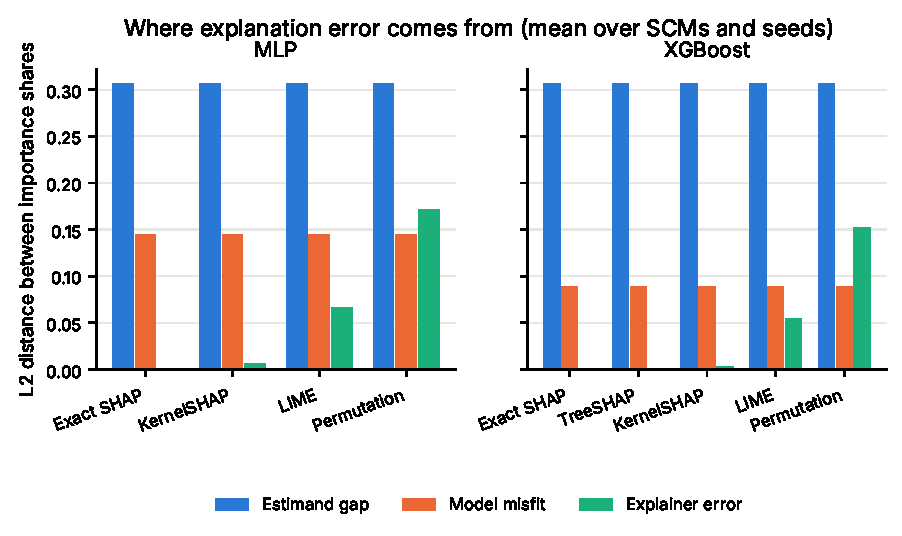
\includegraphics[width=\columnwidth]{fig_error_decomposition_share}
\caption{Share-space error components per explainer and model, mean over SCMs and seeds. The estimand gap (blue) is identical across explainers by construction; the explainer's own error (green) is the smallest term except for permutation importance.}
\label{fig:decomp}
\end{figure}

\subsection{The estimand gap depends on the causal structure}
\TableGapByFamily
\begin{figure}[t]
\centering
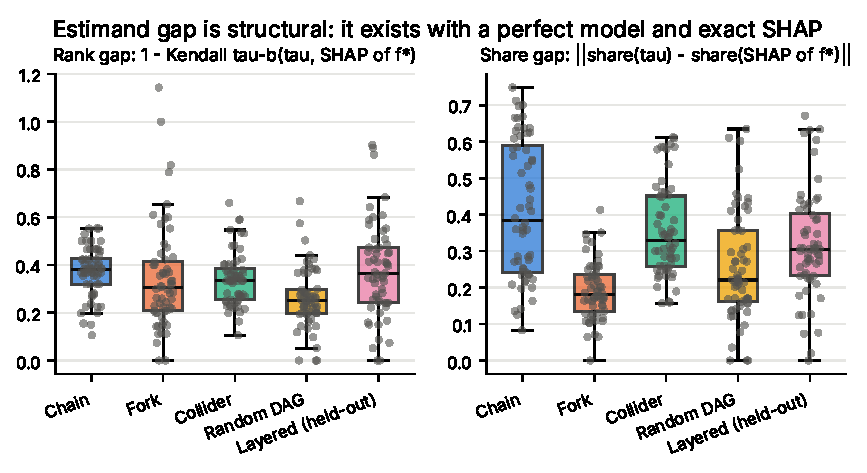
\includegraphics[width=\columnwidth]{fig_estimand_gap_by_family}
\caption{Estimand gap per graph family, one point per SCM (rank space left, share space right). The gap exists for a perfect model and an exact explainer; its size is set by the graph.}
\label{fig:gap}
\end{figure}
Table~\ref{tab:gap} and Fig.~\ref{fig:gap} break the gap down by family. It is largest in share terms for chain-mediation worlds ($0.41$), where on average $38\%$ of the total causal effect sits on features that act on $Y$ only through other features; the true function---and therefore exact SHAP of it---gives them exactly zero, and KernelSHAP and LIME on the fitted models give them $15\%$ and $11\%$. The confounded-fork family shows the opposite failure: non-parents of $Y$ carry only $8\%$ of the causal effect but receive $10\%$ of KernelSHAP's credit, because the fitted models use the confounded proxies. Feature-collider ($0.36$) and layered$^\dagger$ ($0.32$) worlds follow; Erd\H{o}s--R\'enyi DAGs, which have many direct parents of $Y$, have the smallest gap ($0.26$ share, $0.26$ rank). In rank space the ordering is flatter ($0.26$--$0.38$) because a few mediated features with zero attribution already produce several discordant pairs regardless of family. Total rank error of the fitted-model explainers follows the same ordering (chain $0.53$, collider $0.45$, layered$^\dagger$ $0.44$, fork $0.39$, random DAG $0.37$). Every one of the 300 SCMs has a non-zero rank gap.

\subsection{Predicting the error without ground truth}
\TableDiagnosticShare
\TableDiagnosticRank
Tables~\ref{tab:diag_share} and~\ref{tab:diag_rank} report the diagnostic for the two headline targets under the three protocols; Table~\ref{tab:logfo} and Fig.~\ref{fig:logfo} break the LOGFO result down by held-out family.

\emph{Share error is predictable and transfers.} For the share-error target the GBM meta-model reaches a pooled Spearman $\rho$ of $0.65$ ($R^2 = 0.53$) on unseen SCMs from seen families, $0.52$ ($R^2 = 0.33$; bootstrap 95\% CI $[0.43, 0.62]$) under leave-one-graph-family-out, and $0.48$ on the designated held-out layered family. The AUROC for flagging explanations whose share error exceeds the training median is $0.82$, $0.76$ and $0.75$ respectively. All three meta-models behave alike (random forest $0.54$, ridge $0.47$ under LOGFO), so the signal is not an artefact of one learner. Family by family (Table~\ref{tab:logfo}), the meta-model is the best method on every held-out family with $\rho$ between $0.29$ (fork) and $0.81$ (collider) and AUROC between $0.69$ and $0.88$. The best single-signal baseline is test error ($\rho = 0.36$ LOGFO), followed by explainer disagreement ($0.23$); correlation-only, maximum VIF and the constant are at or below zero.

\emph{Rank error is much harder.} For $1 - \tau_b$ the same meta-model reaches $\rho = 0.34$ in-distribution but only $0.22$ under LOGFO and $0.20$ on the layered family, with $R^2$ near zero. Only the disagreement and stability baselines carry any signal for this target ($0.19$ and $0.15$), and the meta-model's gain over them is not significant (Section~\ref{sec:tests}). With at most ten features, Kendall $\tau_b$ takes few distinct values and is dominated by which features receive exact zeros---a structural fact that, as the next section shows, the observables barely see.

\TableLogfoFamily
\begin{figure}[t]
\centering
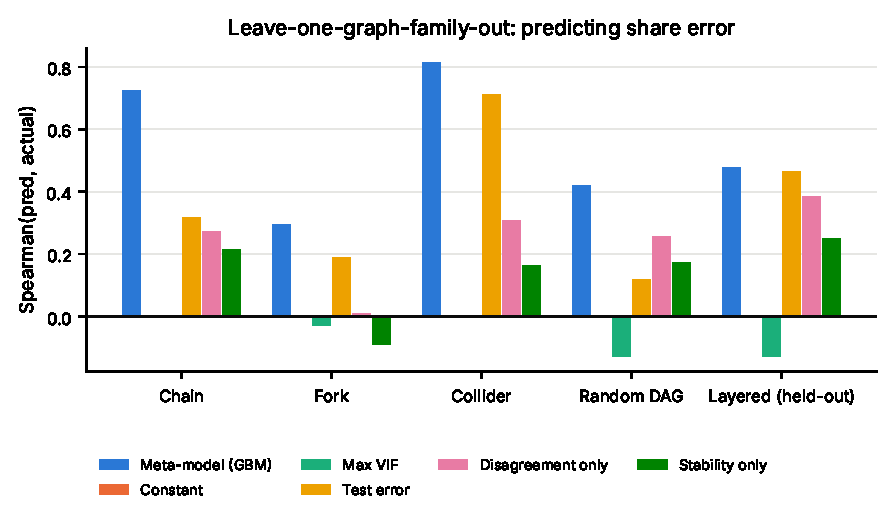
\includegraphics[width=\columnwidth]{fig_logfo_spearman_total_error_share_l2}
\caption{Leave-one-graph-family-out: Spearman correlation between predicted and actual share error on each held-out family, for the GBM meta-model and the single-signal baselines.}
\label{fig:logfo}
\end{figure}
\begin{figure}[t]
\centering
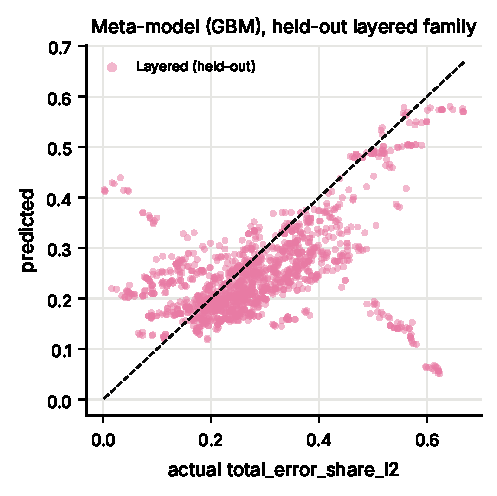
\includegraphics[width=0.8\columnwidth]{fig_pred_vs_actual_designated_split_meta_gbm_total_error_share_l2}
\caption{Predicted vs actual share error on the held-out layered family for the GBM meta-model trained on the four training families.}
\label{fig:pva}
\end{figure}

\subsection{Which part of the error is predictable}
\TableComponents
\begin{figure}[t]
\centering
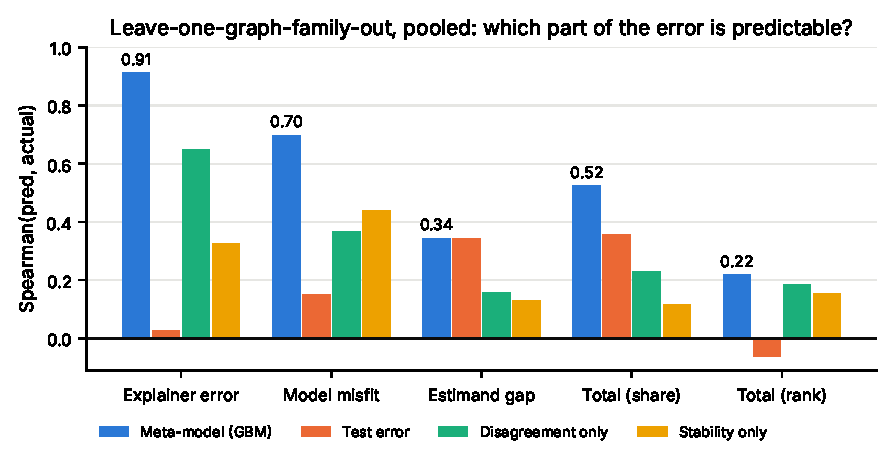
\includegraphics[width=\columnwidth]{fig_component_predictability_logfo_spearman}
\caption{Pooled LOGFO Spearman $\rho$ when each component of the decomposition is the prediction target. The explainer's and the model's contributions are predictable; the structural estimand gap is not.}
\label{fig:components}
\end{figure}
Table~\ref{tab:components} and Fig.~\ref{fig:components} repeat the experiment with each component of~\eqref{eq:decomp} as the target. The ordering is stark. \emph{Explainer error} is almost perfectly predictable ($\rho = 0.91$, $R^2 = 0.98$ under LOGFO): disagreement between explainers run on the same model accounts for most of it on its own ($\rho = 0.65$), with the LIME indicator and sign consistency next. \emph{Model misfit} is well predicted ($\rho = 0.70$, $R^2 = 0.59$), and here the combination matters: test error alone gives $0.15$ and disagreement alone $0.37$, while the meta-model's most important inputs are the disagreement between the XGBoost and MLP attributions, the model indicator, the top-1 share and the seed stability. The \emph{estimand gap}, the largest component, is the least predictable ($\rho = 0.34$, $R^2 = 0.11$), and the meta-model does no better than test error alone ($0.34$); on the layered family it is worse ($0.38$ vs $0.49$). What signal exists comes from the mean feature--outcome correlation and mutual information and from attribution concentration.

The reading is simple. The two components a practitioner could act on---fit the model better, use a better explainer---are the ones the observables reveal. The component that dominates the total is set by which correlated inputs are causes, mediators or proxies of $Y$, and nothing in the observational data, the fitted model or the attributions distinguishes those cases. Because the gap dominates, the total share error is only moderately predictable and the rank error, which is almost entirely gap, hardly at all.

\subsection{Is the gain over the baselines real?}
\label{sec:tests}
\TablePairedTests
Table~\ref{tab:tests} gives the paired comparisons for the share-error target. Under LOGFO the meta-model beats every baseline: against the strongest, test error, the Spearman gain is $0.17$ with a 95\% cluster-bootstrap interval of $[0.08, 0.25]$, the MAE gain is $0.019$ $[0.012, 0.026]$, the Wilcoxon signed-rank test on per-SCM errors gives $p < 0.001$, and the meta-model has the lower error on $65\%$ of SCMs; against the remaining baselines the gains are larger and all intervals exclude zero. On the layered family alone the picture is weaker: the meta-model beats the constant, correlation, VIF, sample-size and stability baselines ($p \le 0.05$) but is indistinguishable from test error ($\Delta\rho = 0.02$ $[-0.28, 0.28]$, $p = 0.62$) and from disagreement ($p = 0.12$); with 60 SCMs in one family the intervals are wide. For the rank-error target the meta-model's gains over disagreement and stability are not significant under any protocol.

\subsection{Which observables carry the signal}
\TableFeatureImportance
\begin{figure}[t]
\centering
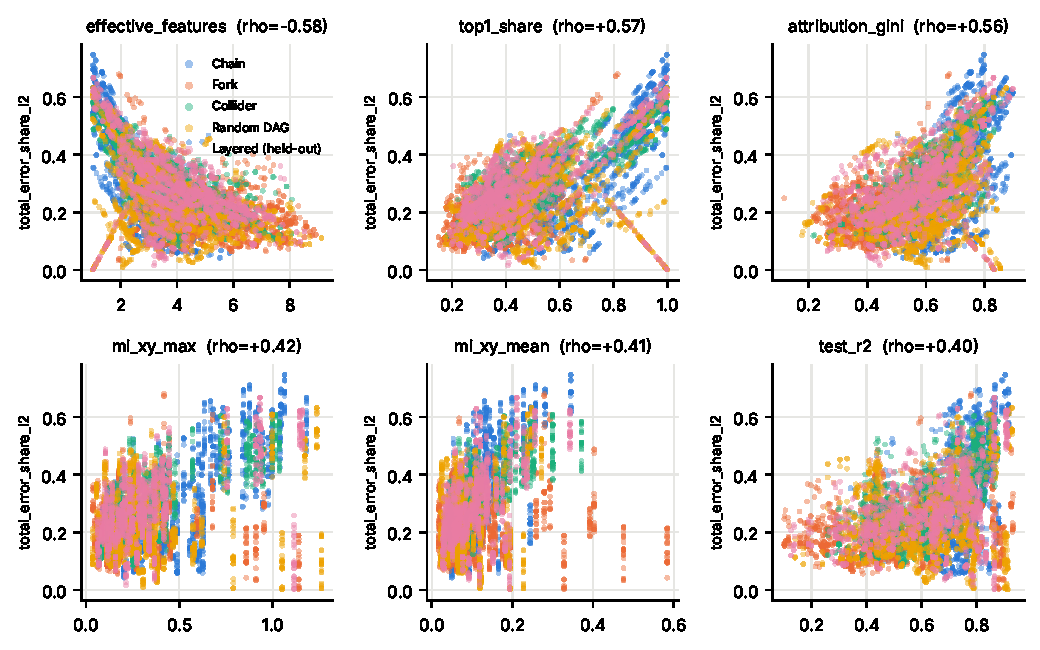
\includegraphics[width=\columnwidth]{fig_observables_vs_total_error_share_l2}
\caption{The six observables most correlated with the share error, one point per explanation, coloured by graph family (Spearman $\rho$ in the panel titles).}
\label{fig:obs}
\end{figure}
Table~\ref{tab:fi} lists the permutation importances of the meta-model trained on the training families and scored on the layered family, and Fig.~\ref{fig:obs} shows the strongest univariate relations. Two groups of observables matter. \emph{Concentration}: explanations that put their mass on few features are far from the causal shares (effective number of features $\rho = -0.58$; top-1 share $+0.57$; Gini $+0.56$). In this benchmark the causal effect is spread along chains and forks while $f^*$, and any model that fits it, concentrates on the direct parents of $Y$. \emph{Feature--outcome association and fit}: the mean feature--outcome $|r|$ has the largest permutation importance ($0.19$), with mutual information with $Y$ ($0.42$ univariate), test $R^2$ ($+0.40$) and cross-model agreement ($+0.39$) close behind. The sign of the fit relation is not the naive one: better-fit outcomes are those with a few dominant direct parents, which is exactly where exact SHAP concentrates credit that the causal effect spreads upstream. Disagreement between explainers ($\rho = 0.34$) and the stability measures add smaller but consistent contributions; maximum VIF, the quantity most often checked in practice, is almost uninformative on its own ($\rho = -0.13$ to $0.05$ across protocols).

\subsection{Ranking SCMs for a fixed explainer}
\TableByMethod
A large part of the variance in error is between explanation methods, which the model and explainer indicators capture trivially. Table~\ref{tab:bymethod} removes that part by scoring predictions within each (model, explainer) subset. The meta-model still ranks SCMs by share error with $\rho = 0.45$--$0.55$ under LOGFO, against $0.27$--$0.47$ for the test-error baseline; the advantage is largest for LIME ($0.45$ vs $0.27$--$0.31$), whose own error is well captured by the disagreement observables, and smallest for permutation importance, whose share error is dominated by its global, loss-based definition.


\section{Discussion}
\subsection{What the results say}
The decomposition reframes a familiar complaint. The literature on causal readings of attributions is usually stated as a warning: SHAP values are not causal effects. Our benchmark puts a number on the warning and locates it. The largest component of the gap between an explanation and the causal effect is not the explainer's approximation and not even the model's imperfection; it is the \emph{definition} of what an attribution measures. This has a practical consequence: investing in a better Shapley estimator (more coalitions, exact TreeSHAP instead of KernelSHAP) reduces the smallest term of~\eqref{eq:decomp} and leaves the dominant one untouched. Only a different estimand---causal or asymmetric Shapley values with a known graph~\cite{heskes2020,frye2020}---can act on it, and those require the very knowledge that is missing in practice.

The second result is more optimistic. Although the gap is structural, its \emph{size} correlates with properties that are visible without the graph. The observables that carry the most signal are of two kinds. Disagreement signals (between explainers on the same model, and between the two model families for the same explainer) are high exactly when the fitted response surface is ambiguous about which correlated inputs to credit, which is also when the credit assignment is most likely to depart from the interventional effect. Fit and concentration signals (test $R^2$, prediction spread, attribution Gini) indicate how much of the outcome the model captures and how many features it leans on; a model that spreads credit widely over correlated inputs has more room to misrank them. Multicollinearity by itself, the signal practitioners most often check, is comparatively weak on its own but useful in combination.

The diagnostic transfers across graph families because it is not learning the families: it has no access to the family label, the mediation share or the presence of confounding, and the LOGFO protocol removes the held-out family's structure from training entirely. What it learns is a mapping from symptoms to error that the five families share, which is the property a diagnostic needs if it is to be used on data whose causal structure is unknown.

\subsection{Limitations}
\textbf{Scope of the benchmark.} All SCMs are small ($d \le 10$, so that exact Shapley values can be enumerated), have additive Gaussian noise, a single continuous outcome, and come from five hand-designed families. Real tabular data has categorical features, heteroscedastic noise, selection effects and far more features. The diagnostic is calibrated to the benchmark's distribution of situations; it should be re-trained or at least re-validated before being trusted elsewhere, and the semi-synthetic checks we planned (IHDP, Adult Income, California Housing) remain future work.

\textbf{Choice of estimand.} We measure error against one causal quantity, the total effect of a unit-standard-deviation shift. Direct effects, binary treatments, or effects on a conditional sub-population would give different estimand gaps, and some would be closer to what interventional SHAP measures. The decomposition itself does not depend on this choice; the numbers do.

\textbf{What the diagnostic does and does not do.} It predicts how far an explanation is likely to be from the causal ranking; it does not say which features are misranked or what the correct ranking is. A high predicted error is a reason to seek domain knowledge or an experiment, not a correction. It is also a regression on the explanation's error magnitude; we report AUROC for a median split as a convenience for a warning threshold, not as a calibrated probability.

\textbf{Dependence between rows.} Rows that share an SCM share data and ground truth. All evaluation is grouped by SCM and all tests resample SCMs, but the effective sample size for the family-level conclusions is 60 SCMs per family, and the per-family LOGFO numbers should be read with that in mind.

\textbf{Compute.} Exact Shapley values of the fitted model cost $100 \times 50 \times 2^d$ model evaluations per seed; the full run (300 SCMs, 2 models, 3 seeds, 5 explainers, perturbation re-explanations) takes about three hours on two CPU cores. Larger $d$ would need sampled-coalition oracles, which would blur the line between $\Phi(f)$ and $\hat E$.


\section{Conclusion}
We set out to test whether the error of a feature attribution, measured against the causal effect it is commonly read as, can be predicted without causal ground truth. On a benchmark of 300 synthetic causal worlds the answer has two halves. Most of the error is structural: exact Shapley values of the true outcome function already misallocate a third of the importance mass relative to the total interventional effect, and better explainers do not change that. The part of the error that observable signals can see is the part contributed by the fitted model and the explainer; a gradient-boosted diagnostic predicts those components well, transfers to graph families it never saw, and beats every single-signal practitioner baseline for the total share error. The structural estimand gap, however, is largely invisible to the same signals, and the feature ranking error that follows from it is hardly predictable. The practical conclusion is a modest one: observable diagnostics can tell a practitioner when to distrust an explanation because the model or the explainer is at fault, but they cannot substitute for the causal knowledge that decides whether a Shapley attribution answers the interventional question at all. Code, the benchmark, the notebook and all tables are available at \url{https://github.com/stacktrace-bhuvi/datasphere}.

\section*{Contributions}
B.S.K.: SCM generation, interventional engine, oracle SHAP, data contracts. M.S.: model training, explainer wrappers, attribution persistence. P.L.B.R.: error metrics, decomposition, error-table builder and summary tables. D.S.: observables, diagnostic meta-models, baselines, evaluation protocols, statistical tests and figures.

\begin{thebibliography}{00}
\bibitem{lundberg2017} S.~M. Lundberg and S.-I. Lee, ``A unified approach to interpreting model predictions,'' in \emph{Advances in Neural Information Processing Systems 30}, 2017.
\bibitem{ribeiro2016} M.~T. Ribeiro, S. Singh, and C. Guestrin, ``\,`Why should I trust you?': Explaining the predictions of any classifier,'' in \emph{Proc.\ 22nd ACM SIGKDD}, 2016, pp.~1135--1144.
\bibitem{janzing2020} D. Janzing, L. Minorics, and P. Bl\"obaum, ``Feature relevance quantification in explainable AI: A causal problem,'' in \emph{Proc.\ 23rd AISTATS}, PMLR 108, 2020, pp.~2907--2916.
\bibitem{krishna2022} S. Krishna, T. Han, A. Gu, J. Pombra, S. Jabbari, S. Wu, and H. Lakkaraju, ``The disagreement problem in explainable machine learning: A practitioner's perspective,'' \emph{arXiv:2202.01602}, 2022.
\bibitem{agarwal2022} C. Agarwal, S. Krishna, E. Saxena, M. Pawelczyk, N. Johnson, I. Puri, M. Zitnik, and H. Lakkaraju, ``OpenXAI: Towards a transparent evaluation of model explanations,'' in \emph{Advances in Neural Information Processing Systems 35, Datasets and Benchmarks Track}, 2022.
\bibitem{breiman2001} L. Breiman, ``Random forests,'' \emph{Machine Learning}, vol.~45, no.~1, pp.~5--32, 2001.
\bibitem{heskes2020} T. Heskes, E. Sijben, I.~G. Bucur, and T. Claassen, ``Causal Shapley values: Exploiting causal knowledge to explain individual predictions of complex models,'' in \emph{Advances in Neural Information Processing Systems 33}, 2020.
\bibitem{frye2020} C. Frye, C. Rowat, and I. Feige, ``Asymmetric Shapley values: Incorporating causal knowledge into model-agnostic explainability,'' in \emph{Advances in Neural Information Processing Systems 33}, 2020.
\bibitem{alvarez2018} D. Alvarez-Melis and T.~S. Jaakkola, ``On the robustness of interpretability methods,'' in \emph{ICML Workshop on Human Interpretability in Machine Learning}, 2018.
\bibitem{pearl2009} J. Pearl, \emph{Causality: Models, Reasoning, and Inference}, 2nd~ed. Cambridge University Press, 2009.
\bibitem{chen2016} T. Chen and C. Guestrin, ``XGBoost: A scalable tree boosting system,'' in \emph{Proc.\ 22nd ACM SIGKDD}, 2016, pp.~785--794.
\end{thebibliography}

\end{document}
